% ::setlocal makeprg=cd\ presentazione\ &&\ pdflatex\ -interaction=batchmode\ main.tex\ &&\ okular\ main.pdf\ &

\section{Capitolo 2}

\begin{frame}{Simulazione}

    con RK4

\end{frame}


\begin{frame}{Video on the computer}
    \centering
    \movie[externalviewer]{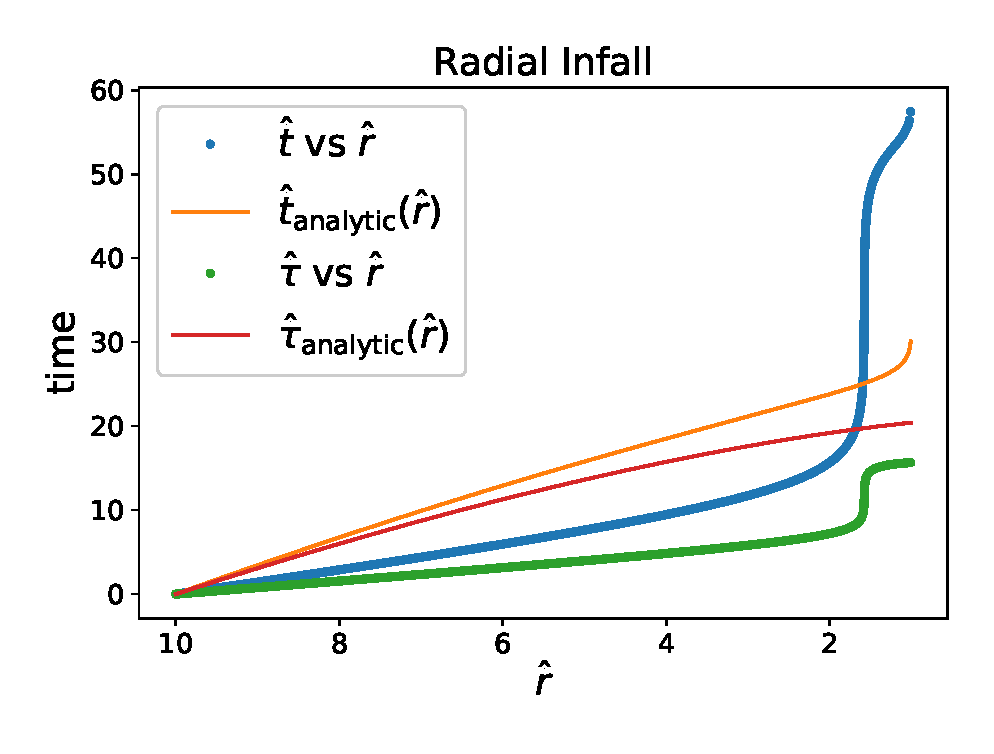
\includegraphics[width=\textheight, keepaspectratio]
    {Videos/infall.png}}{Videos/infall.mov}
\end{frame}


\begin{frame}{Video on the computer}
    \centering
    \movie[externalviewer]{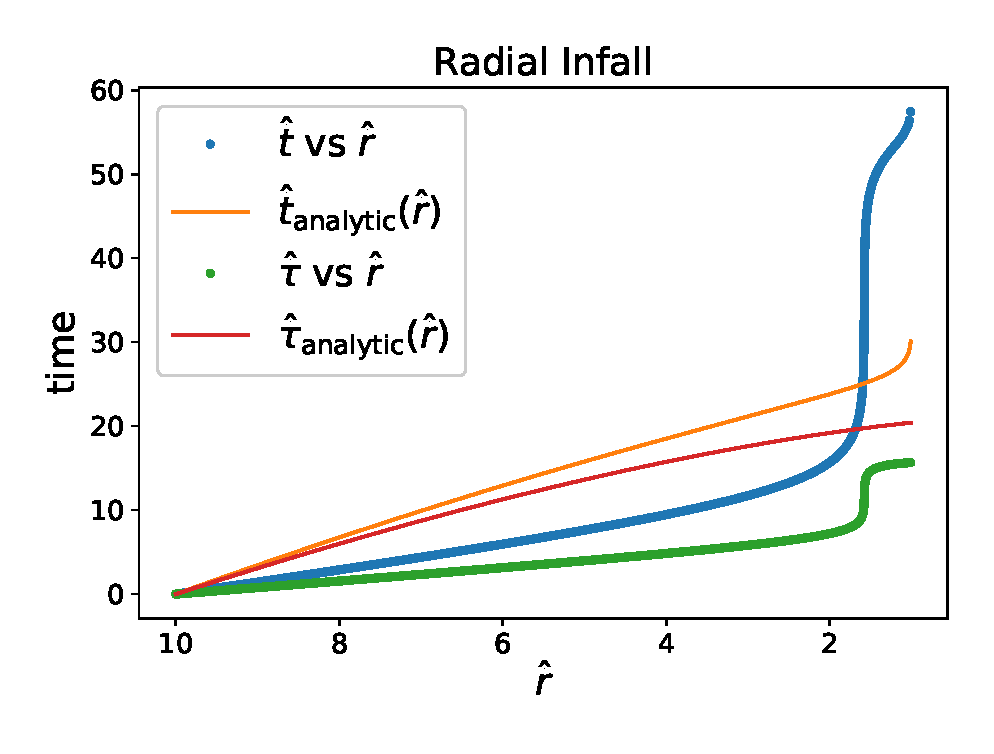
\includegraphics[width=\textheight, keepaspectratio]
    {Videos/infall.png}}{Videos/infall.mp4}
\end{frame}


\begin{frame}{Video on the computer}
    \centering
    \movie[externalviewer]{\includegraphics[width=\textheight, keepaspectratio]
    {Videos/volevi.png}}{Videos/volevi.mov}
\end{frame}


\begin{frame}{Video on the computer}
    \centering
    \movie[externalviewer]{\includegraphics[width=\textheight, keepaspectratio]
    {Videos/precession.png}}{Videos/precession.mp4}
\end{frame}


\begin{frame}{Video on the computer}
    \centering
    \movie[externalviewer]{\includegraphics[width=\textheight, keepaspectratio]
    {Videos/precession2.png}}{Videos/precession2.mp4}
\end{frame}


\begin{frame}{Video on the computer}
    \centering
    \movie[externalviewer]{\includegraphics[width=\textheight, keepaspectratio]
    {Videos/precession2.png}}{Videos/precession2.MOV}
\end{frame}


\begin{frame}{Video on the computer}
    \centering
    \movie[externalviewer]{\includegraphics[width=\textheight, keepaspectratio]
    {Videos/precession_ani.png}}{Videos/precession_ani.mov}
\end{frame}
